\chapter{Implementacja}
Podczas pracowni dyplomowej nie miałem wiele czasu na implementację biblioteki. Udało mi się wykonać jedynie prototyp rozwiązania w~postaci uproszczonego wykresu słupkowego. Jest to rozwiązanie niepełne, które jednak implementuje najważniejsze mechanizmy z~rozdziału \textit{Projekt}~\ref{chap:proj}. 

Poniżej opisuję narzędzia, które wykorzystałem podczas prac nad biblioteką. Następnie opisuję najciekawsze szczegóły implementacyjne oraz odstąpienia od projektu. Na koniec przedstawiam zaimplementowany przeze mnie wykres słupkowy.

\section{Wykorzystane narzędzia}
Do stworzenia tej pracy inżynierskiej wykorzystałem najlepiej znane mi narzędzia. Ze wszystkich opisanych poniżej, tylko Qt~5 było dla mnie pewną nowością. Z~pozostałych korzystam zarówno w~pracy, jak i~na uczelni.
 
\subsubsection{Qt 5}
Najnowsza dostępna wersja Qt to 5.1. Nowa odsłona dostarcza programistom szereg usprawnień oraz modułów, m.in. do obsługi formatu JSON. Jednak głównym punktem Qt~5 jest nowa implementacja Qt~Quick. 

Do implementacji Qt~Quick~2 wykorzystano OpenGL i~SceneGraph, co znacznie poprawiło wydajność tego systemu. Qt~5 rozpoczęło też nowy kierunek rozwoju aplikacji wykorzystujących Qt. Qt~Quick jest promowany jako zalecany sposób tworzenia interfejsów użytkownika. Docelowo aplikacje Qt mają być podzielone na GUI napisane w~QML oraz logikę zaprogramowaną w~C++.

\subsubsection{Qt Creator}
Qt~Creator to zintegrowane środowisko programistyczne przeznaczone głównie dla języków C++, QML oraz JavaScript. Jego edytor tekstowy zawiera takie udogodnienia jak kolorowanie składni czy narzędzia do refaktoryzacji kodu. Qt~Creator zawiera także wtyczkę do tworzenia graficznych interfejsów użytkownika. Korzystanie z~Designera jest proste i~intuicyjne, a~proste GUI można w~dużej mierze ,,wyklikać''.

Do budowania i~debugowania Qt~Creator wykorzystuje domyślne oprogramowanie danej platformy, np. kompilator gcc i~debuger gdb na systemie Linux. Creator posiada graficzny interfejs do debuggera, który w~znaczący sposób upraszcza procesz debugowania.

Qt~Creator posiada również wtyczki integrujące go z~najpopularniejszymi systemami kontroli wersji. Lista wspieranych systemów:
\begin{itemize}
\item{Bazaar,}
\item{CVS,}
\item{Git,}
\item{Mercurial,}
\item{Perforce,}
\item{Subversion.}
\end{itemize}

\subsubsection{Subversion}
Subversion to scentralizowany system kontroli wersji będący następcą systemu CVS. Repozytorium SVN założyłem w~serwisie Google Code~\footnote{http://code.google.com/intl/pl/}, pod adresem \url{http://code.google.com/p/qt-west-charts/}.

\subsubsection{Kubuntu 12.04 LTS}
Kubuntu to pochodna Ubuntu, korzystająca z~KDE -- graficznego środowiska, zbudowanego w~oparciu o~bibliteki Qt. ,,Kubuntu oznacza \textit{w stronę ludzkości} w języku bemba''~\footnote{Kubuntu \url{http://pl.wikipedia.org/wiki/Kubuntu}} -- jest to cytat, który jednoznacznie wskazuje co jest celem istnienia tej dystrybucji Linuxa.

Kubuntu jest udostępniane z~bogatym zbiorem aplikacji biurowych, multimedialnych oraz wielu innych. Najpopularniejsze aplikacje, które są dostarczane wraz z~systemem Kubuntu to LibreOffice i~GIMP. 


\section{Szczegóły implementacyjne}
Rozdział \textit{Projekt}~\ref{chap:proj} nie jest bardzo precyzyjną dokumentacją techniczną. Celem tego rozdziału było przedstawienie pewnych rozwiązań architektonicznych, których uszczegółowienie było możliwe dopiero na etapie implementacji, gdyż, jako projektant, nie byłem w~stanie przewidzieć wszystkich trudności związanych z~implementacją. Ten podrozdział służy uszczegółowieniu pewnych kwestii, które dotychczas nie zostały wystarczająco rozwinięte.

\subsection{Nieidealna separacja}
W mojej bibliotece odseparowałem warstwę prezentacji od warstwy danych poprzez podział na wykres oraz model. Wykres odpowiada za prezentację danych, których źródłem jest model. Dany model może być źródłem danych dla wielu wykresów.

Separacja tych dwóch warstw nie jest jednak idealna, gdyż model zawiera takie informacje jak kolor czy tytuł próbki. Uniemożliwia to zaprezentowanie tych samych danych w~dwóch wykresach za pomocą różnych palet kolorów. Podejście to ma jednak swoje plusy. Sprawia, że użytkownik nie musi ,,zaglądać'' do wewnętrznych elementów wykresu. Stworzenie prostego wykresu ogranicza się do powołania jego instancji i~podłączenia źródła wypełnionego danymi. Taka prostota jest szczególnie porządana w~przypadku deklaratywnego języka, jakim jest QML.

Na myśl przyszło mi kilka rozwiązań tego problemu, ale wydają mi się one albo niezbyt eleganckie, albo nazbyt skomplikowane. Zdaje się, że najwłaściwszym byłoby wprowadzenie elementu takiego jak delegat~\footnote{Delegat \url{http://qt-project.org/doc/qt-5.0/qtwidgets/model-view-\newline programming.html\#delegates}} w~architekturze \textit{Model-Widok}. Byłoby to odpowiednie rozwiązanie dla doświadczonych programistów, chcących tworzyć bardziej zaawansowane wykresy.

Z uwagi na prostotę użycia zdecydowałem się pozostać przy obecnym rozwiązaniu. Jeśli wyżej opisany problem okaże się palący dla użytkowników, będę zmuszony wprowadzić mechanizm delegatów.

\subsection{Elastyczność źródła danych}\label{sub:flexible}
Dzięki zastosowaniu dwóch ciekawych technik programistycznych osiągnąłem bardzo dużą elastyczność przy wyborze źródła danych dla wykresu. Pierwsza z~nich, to przyjmowanie jako model obiektu \textit{QVariant}. Druga to wprowadzenie adptera modelu~\ref{sec:zrodla}, który jest mostem~\ref{sec:most}.

Dodanie nowego źródła danych ogarnicza się do zarejestrowania klasy źródła jako \textit{QVariant} oraz obsłużenia tego źródła w~ciele mostu. Uchwyt mostu pozostaje niezmieniony, dzięki czemu wprowadzenie nowego źródła danych nie spowoduje ponownej kompilacji całej biblioteki oraz aplikacji z~niej korzystajacych, a~jedynie ponowne linkowanie.

\subsection{Wtyczka Qt~Quick}
Rozszerzenia Qt~Quick są realizowane poprzez system wtyczek, które są ładowane na starcie aplikacji. Głównym celem takiej wtyczki jest zarejestrowanie wszystkich klas C++, które później mają być dostępne w~QML. Wtyczka musi dziedziczyć po klasie \textit{QQmlExtensionPlugin}, a~rejestrowane klasy muszą być pochodnymi \textit{QObject}.

W przypadku mojego projektu, wtyczka zawiera adaptery do klas biblioteki, realizujących właściwą funkcjonalność. Zdecydowałem się zastosować takie podejście z~kilku powodów.

Po pierwsze, nie wszystkie klasy Qt są dostępne z~poziomu QML. Najlepszym przykładem jest pędzel, czyli obiekt klasy \textit{QBrush}. Programiści C++ mają możliwość ustawienia wszystkich parametrów pędzla odpowiedzialnego za odmalowanie tła wykresu. Z~poziomu QML udostępniam możliwość ustawienia tylko koloru pędzla.

Kolejny argument przemawiający za moim rozwiązaniem, to uniknięcie przesadnie rozbudowanych interfejsów. Udostępnienie wszystkich parametrów pędzla za pomocą systemu właściwości spowodowałoby drastyczne rozbudowanie interfejsu danej klasy.

Ostatnim, przeważającym argumentem jest fakt, że właśnie takie podejście jest standardowym rozwiązaniem stosowanym przy eksponowaniu klas C++ do Qt~Quick. W~QML udostępniane są jedynie najważniejsze parametry, np. kolor pędzla, a~te mniej znaczące są pomijane. Wydruk~\ref{code:qoc:adapter} zawiera przykładowy adapter znajdujący się we wtyczce Qt~Quick mojej biblioteki.

\begin{lstlisting}[caption=Adapter klasy QocAbstractChart, label=code:qoc:adapter]
class QOC_QUICK_API QocQuickAbstractChart : public QocAbstractChart
{
	Q_OBJECT
	Q_PROPERTY(QColor backgroundColor 
		   READ backgroundColor 
		   WRITE setBackgroundColor 
		   NOTIFY backgroundColorChanged)
	...
}
\end{lstlisting}


\subsection{Biblioteka na platformie Windows}
Podczas budowania dowolnej biblioteki na platformie Windows, niezbędne jest wyeksportowanie symboli. Proces ten muszą przejść wszystkie elementy, które mają być dostępne dla klientów danej biblioteki. W~przypadku mojego projektu eksportowane były jedynie nagłówki klas, jednak mogą to być również globalne funkcje lub zmienne. Eksport symboli odbywa się za pomocą dostarczanych przez Qt makrodefinicji, których wykorzystanie w~mojej bibliotece przedstawiam na wydrukach~\ref{code:qoc:global} i~\ref{code:qoc:klasa}.

\begin{lstlisting}[caption=Zawartość pliku qoc\_global.h, label=code:qoc:global]
#include <QtCore/QtGlobal>

#if defined(QOC_LIBRARY)
#  define QOC_API Q_DECL_EXPORT
#else
#  define QOC_API Q_DECL_IMPORT
#endif
\end{lstlisting}

\begin{lstlisting}[caption=Eksport klasy QocAbstractChart, label=code:qoc:klasa]
#include "qoc_global.h"

class QOC_API QocAbstractChart : public QObject
{
   ...
}
\end{lstlisting}


Dzięki dodadniu do pliku projektu instrukcji: \textit{DEFINES +=  QOC\_LIBRARY}, podczas budowania biblioteki makro \textit{QOC\_API} powoduje wyeksportowanie symboli. Z~kolei dla klientów biblioteki makro po rozwinięciu przez preprocesor spowoduje ich import.


\section{Odstępstwa od projektu}
Faza implementacji zweryfikowała założenia projektowe. Część z~nich się obroniła, pozostałe musiałem nagiąć bądź całkowicie z~nich zrezygnować. Poniżej opisuję wszystkie sytuacje, w~których postępowałem niezgodnie z~projektem.

\subsection{Oszczędne korzystanie ze wzorca Most}
Zmniejszenie zależności między plikami poprzez wykorzystanie wzorca mostu, opisane w~rozdziale~\ref{sec:most}, dostarczyło mi dość dużo dodatkowej pracy. Dlatego postanowiłem korzystać z~tego rozwiązania jedynie tam, gdzie ma to sens.

Miejscami, w~których dodatkowa praca przeznaczona na stworzenie mostu się zwraca, są klasy przeznaczone do rozbudowywanie. Są to klasy bazowe takie jak \textit{QocAbstractChart} albo węzły takie jak \textit{QocAdaptorModel}. Korzyści wynikające z~zastosowania mostu w~takim miejscu opisałem w~punkcie~\ref{sub:flexible}. Natomiast proste klasy, które nie są przeznaczone do dziedziczenia, jak \textit{QocAxis}, nie zostały zaimplementowane jako most.


\section{Prototyp wykresu słupkowego}
Udało mi się zaimplementować rdzeń wykresu słupkowego. Z~uwagi na niewielką ilość czasu pominąłem niektóre rozwiązania architektoniczne, jednak zachowałem najważniejsze z~nich, takie jak separacja danych od prezentacji czy podział wykresu na warstwy. 

W~obecnym stanie, za pomocą wykresu słupkowego można prezentować dane tylko z~jednej serii. Możliwa jest animacja elementów wykresu. W~przykładowym programie zaanimowałem wysokość słupków. Wykres podpiąłem do dwóch widoków -- widgetu oraz elementu QML. Poniżej prezentuję kilka zrzutów z~ekranu, zawierających ten wykres. 

\begin{figure}[H]
\centering
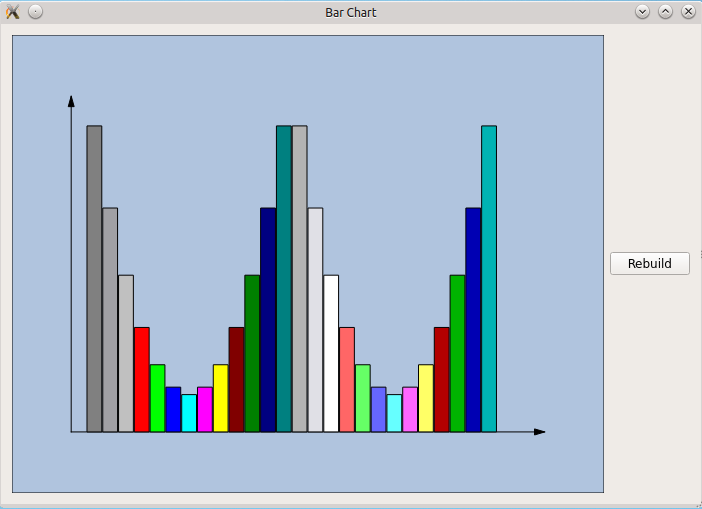
\includegraphics[scale=0.5]{img/BarChart_kubuntu.png}
\caption{Wykres w widgecie -- Kubuntu 12.04}\label{rys:bar:kubuntu}
\end{figure}

TODO: Windows 7 \& Qt~Quick

%\section{Tworzenie biblioteki współdzielonej}
%Biblioteka współdzielona to rodzaj biblioteki dynamicznej, czyli biblioteki łączonej z~programem dopiero w~trakcie jego uruchamiania. Przy pierwszym uruchomieniu programu korzystającego z~danej biblioteki współdzielonej, biblioteka ta zostaje załadowana w~całości do pamięci. Od tej pory wszystkie programy, będą mogły korzystać z~tej biblioteki bez ponownego jej ładowania. W~systemach Unixowych biblioteki dynamiczne mają rozszerzenie .so, a~w~systemach Windows .dll.

%Qt udostępnia nam stosunkowo prosty sposób na tworzenie bibliotek dynamicznych.

%\subsection{Symbole}
%Wszelkie funkcje, zmienne i klasy zawarte w~bibliotece, które są przeznaczone do użytku dla klientów biblioteki są nazywane publicznymi symbolami i~muszą zostać wyeksportowane, czyli upublicznione podczas kompilacji biblioteki. Zazwyczaj domyślne zachowanie kompilatorów to ukrywanie wszystkich symboli. Aby stały się one dostępne dla klientów biblioteki, trzeba to otwarcie zasygnalizować podczas kompilacji. Natomiast na niektórych platformach osobnych instrukcji wymaga ukrycie symboli.

%\subsection{Eksport -- Import}
%Rozwiązaniem obu problemów są dwa makra dostarczane przez Qt, które muszą zostać dodane do deklaracji symboli:
%\begin{itemize}
%\item{Q\_DECL\_EXPORT -- przy kompilacji dynamicznej biblioteki}
%\item{Q\_DECL\_IMPORT -- przy kompilacji klienta korzystającego z~biblioteki}
%\end{itemize}

%\subsection{Uniwersalne makro}
%Teraz trzeba się upewnić, że odpowiednie makro zostanie wykorzystane w~odpowiednim momencie. Typowym rozwiązaniem jest dodanie specjalnego pliku nagłówkowego, np. \textit{foolib\_global.h}. Plik ten musi zawierać kod preprocesora realizujący następującą sztuczkę:
%\begin{lstlisting}[caption=Warunkowa kompilacja, label=code:kompilacja:warunkowa]
%#include <QtCore/QtGlobal>

%#if defined(FOOLIB_LIBRARY)
%#  define FOOLIB_API Q_DECL_EXPORT
%#else
%#  define FOOLIB_API Q_DECL_IMPORT
%#endif
%\end{lstlisting}

%Jak widać, w~zależności od tego czy istnieje makro \textit{FOOLIB\_LIBRARY}, makro \textit{FOOLIB\_API} posłuży do eksportowania albo importowania symboli biblioteki \textit{FooLib}. Makro \textit{FOOLIB\_LIBRARY} zostanie zdefiniowane tylko i~wyłącznie w~pliku projektu biblioteki \textit{FooLib}. Tylko wtedy będziemy mieli pewność, że nasza biblioteka będzie poprawnie linkowana. W~pliku .pro należy dodać instrukcję: \textit{DEFINES +=  FOOLIB\_LIBRARY}.

%\subsection{Wykorzystanie makra}
%We wszystkich plikach nagłówkowych biblioteki, deklaracje symboli muszą zostać uzupełnione o~nasze makro:

%\begin{lstlisting}[caption=Eksport symboli, label=code:eksport:sym]
%#include "foolib_global.h"

%FOOLIB_API void foo();
%class FOOLIB_API Foo...
%\end{lstlisting}

